\documentclass[aspectratio=1610,11pt]{beamer}
\geometry{paperwidth=20cm,paperheight=11.25cm}
\usepackage[T1]{fontenc}
\usepackage{tgpagella}
\usepackage{tgheros}
\usepackage{tikz}
\usepackage{booktabs}
\usepackage{pgfpages}
\usetikzlibrary{arrows.meta,positioning,calc,shapes.geometric,decorations.pathreplacing}
\usefonttheme{professionalfonts}
\definecolor{Ink}{RGB}{24,47,57}
\definecolor{Teal}{RGB}{21,102,121}
\definecolor{Rust}{RGB}{181,83,48}
\definecolor{Paper}{RGB}{249,248,244}
\definecolor{Mist}{RGB}{231,239,239}
\definecolor{CardFill}{RGB}{210,229,232}
\definecolor{PCardFill}{RGB}{225,229,211}
\definecolor{Warm}{RGB}{249,233,219}
\definecolor{Muted}{RGB}{91,104,110}
\definecolor{Olive}{RGB}{104,116,56}
\hyphenpenalty=10000 \exhyphenpenalty=10000
\setbeamercolor{normal text}{fg=Ink,bg=Paper}
\setbeamercolor{frametitle}{fg=Ink,bg=Paper}
\setbeamercolor{structure}{fg=Teal}
\setbeamercolor{paperbox}{fg=Ink,bg=Mist}
\setbeamercolor{conclusion}{fg=Ink,bg=Warm}
\setbeamerfont{frametitle}{family=\rmfamily,size=\LARGE}
\setbeamerfont{normal text}{family=\sffamily}
\setbeamersize{text margin left=7mm,text margin right=7mm}
\setbeamertemplate{navigation symbols}{}
\setbeamertemplate{itemize item}{\color{Teal}\raisebox{1pt}{\tiny$\blacksquare$}}
\setbeamertemplate{frametitle}{\vspace{4mm}\insertframetitle\par\vspace{1mm}
  {\color{Teal}\rule{14mm}{1.1pt}}\vspace{1mm}}
% \setbeamertemplate{footline}{\hspace{7mm}{\color{Muted}\fontsize{6.7}{8}\selectfont
%   PATHFINDER\quad /\quad IQ LAB, LIP6\quad /\quad 17 SEPTEMBER 2026}
%   \hfill{\color{Muted}\fontsize{7}{8}\selectfont
%   \ifnum\value{framenumber}>13 BACKUP\else\insertframenumber\,/\,13\fi}\hspace{7mm}\vspace{3mm}}
\setbeamertemplate{footline}{\hspace{7mm}{\color{Muted}\fontsize{6.7}{8}\selectfont
  % PATHFINDER\quad /\quad IQ LAB, LIP6\quad /\quad 17 SEPTEMBER 2026}
  % \hfill{\color{Muted}\fontsize{7}{8}\selectfont
  \ifnum\value{framenumber}>14 BACKUP\else\insertframenumber\,/\,14\fi}\hspace{7mm}\vspace{3mm}}
\hypersetup{pdftitle={Pathfinder: from seminar questions to research},
  pdfauthor={Vincent Danos, Elham Kashefi, William Waites},colorlinks=true,urlcolor=Teal}
\ifdefined\SpeakerNotes
  \setbeameroption{show notes on second screen=right}
\else
  \setbeameroption{hide notes}
\fi
\newcommand{\assetdir}{assets/2026-09-16-200514}
\newcommand{\JulienRows}{82}
\newcommand{\JulienColumns}{82}
\newcommand{\JulienPairs}{6,724}
\newcommand{\JulienScored}{5,822}
\newcommand{\JulienMissing}{902}
\newcommand{\QSLRows}{88}
\newcommand{\QSLColumns}{124}
\newcommand{\QSLPairs}{10,912}
\newcommand{\QSLScored}{10,912}
\newcommand{\ScenarioTotal}{601}
\newcommand{\RecordedInput}{51.0}
\newcommand{\RecordedOutput}{1.82}
\newcommand{\CampaignSpan}{43.7}
\newcommand{\AgentHours}{8.1}
\newcommand{\ScanCost}{3.75}
\newcommand{\ResearchCost}{410.56}
\newcommand{\ManuscriptCost}{116.11}
\newcommand{\AccountCost}{70.52}

% a quiet line under the title: sentence case, no capitals
\newcommand{\kicker}[1]{{\color{Muted}\fontsize{9}{11}\selectfont #1\par}\vspace{2mm}}
\newcommand{\smallprint}[1]{\par{\color{Muted}\fontsize{8}{10}\selectfont #1\par}}
% the slide's conclusion, anchored to the bottom of the frame, with a rust rule on its left
\newcommand{\takeaway}[1]{\par\vfill\noindent{\setlength{\fboxsep}{0pt}\colorbox{Rust}{\hspace*{2.4pt}%
  {\setlength{\fboxsep}{7pt}\colorbox{Warm}{\parbox{\dimexpr\linewidth-2.4pt-14pt\relax}{%
  \raggedright\fontsize{10.5}{13.5}\selectfont #1}}}}}\par}
% narrative stage labels inside a case study
\newcommand{\stage}[2][Teal]{{\color{#1}\fontsize{10}{12}\selectfont\bfseries #2}}
% one line of a dialogue: speaker in colour, words beside
\newcommand{\dline}[3]{\par\noindent\makebox[17mm][l]{\color{#1}\fontsize{13}{17}\selectfont\bfseries #2}%
  {\color{#1!78!Ink}\parbox[t]{\dimexpr\linewidth-17mm\relax}{\fontsize{13}{17}\selectfont\raggedright #3}}\par\vspace{4mm}}
% a source paper: corpus colour on the left edge and on its label (Q teal, P olive)
\newcommand{\corpuscard}[6]{\begin{tikzpicture}
  \node[fill=#1,rounded corners=2.5pt,inner xsep=8pt,inner ysep=5pt,outer sep=0pt,
    text width=\dimexpr\linewidth-16pt\relax,align=left] (c) {%
      \begin{minipage}[t][35pt][t]{\linewidth}
      {\fontsize{9}{11}\selectfont{\color{#2}\bfseries #3}\enspace{\bfseries #4}\par}\vspace{1.5pt}
      {\color{Ink}\fontsize{8.6}{10.6}\selectfont #5\par #6\par}
      \end{minipage}};
  \begin{scope}\clip[rounded corners=2.5pt] (c.south west) rectangle (c.north east);
    \fill[#2] (c.south west) rectangle ([xshift=2.6pt]c.north west);\end{scope}
  \end{tikzpicture}}
\newcommand{\qcard}[4]{\corpuscard{CardFill}{Teal}{#1}{#2}{#3}{#4}}
\newcommand{\pcard}[4]{\corpuscard{PCardFill}{Olive}{#1}{#2}{#3}{#4}}

% mini abstracts
\newcommand{\Qfour}{\qcard{Q4}{Incentives to report what one knows}
  {Agents may profit by hiding what they know.}
  {Rewards can make truthful reporting worthwhile.}}
\newcommand{\Psix}{\pcard{P6}{An outside judge for a team}
  {A team works together; credit is hard to assign.}
  {An outside AI judges contributions from images.}}
\newcommand{\Qseven}{\qcard{Q7}{Sharing resources}
  {Participants compete for limited resources.}
  {Messages and payments aim to share them well.}}
\newcommand{\Pone}{\pcard{P1}{Learning about bad outcomes}
  {Learn to act while controlling bad outcomes.}
  {Estimate losses in the worst fraction of cases.}}
\newcommand{\Qthree}{\qcard{Q3}{AI agents in a market}
  {AI agents buy and sell in a simulated market.}
  {Their performance is compared with humans.}}
\newcommand{\Pthree}{\pcard{P3}{A critic for the code reviewer}
  {An AI reviews code; a critic challenges its review.}
              {The coding agent then revises the program.}}
\newcommand{\paperpair}[2]{\begin{columns}[T,onlytextwidth]
  \begin{column}{.49\textwidth}#1\end{column}
  \begin{column}{.49\textwidth}#2\end{column}\end{columns}\vspace{2.5mm}}
\newcommand{\connectedpaperpair}[3][connexion]{\begin{columns}[c,onlytextwidth]
  \begin{column}{.445\textwidth}#2\end{column}
  \begin{column}{.09\textwidth}\centering
    \begin{tikzpicture}[baseline=-.5ex]
      \draw[flow] (0,0) -- node[above=2pt,font=\fontsize{6.5}{8}\selectfont,text=Teal] {#1} (1.35,0);
    \end{tikzpicture}
  \end{column}
  \begin{column}{.445\textwidth}#3\end{column}\end{columns}\vspace{2.5mm}}
\tikzset{flow/.style={-{Stealth[length=2mm]},draw=Teal,line width=.8pt},
  state/.style={draw=Teal,fill=Mist,rounded corners=2pt,minimum height=9mm,
    inner sep=5pt,align=center,font=\small},
  paused/.style={state,draw=Rust,fill=Warm},
  lab/.style={font=\scriptsize,fill=Paper,inner sep=2pt,align=center},
  agent/.style={circle,fill=Teal,draw=none,minimum size=5mm,inner sep=0pt}}

\begin{document}

\begin{frame}[plain]
\vspace{7mm}
\kicker{IQ lab, LIP6\qquad 17 September 2026}
\vspace{9mm}
{\rmfamily\fontsize{50}{54}\selectfont Pathfinder}\par\vspace{3mm}
{\rmfamily\fontsize{21}{26}\selectfont From seminar questions\\to research}\par
\vspace{5mm}{\color{Teal}\rule{28mm}{1.5pt}}\par\vspace{9mm}
\begin{minipage}{.6\textwidth}
\begin{columns}[T,onlytextwidth]
  \begin{column}{.3\textwidth}
    {\bfseries Vincent Danos}\par\vspace{1.5mm}
    {\small\color{Muted}CNRS, ENS}
  \end{column}
  \begin{column}{.36\textwidth}
    {\bfseries Elham Kashefi}\par\vspace{1.5mm}
    {\small\color{Muted}CNRS, LIP6\\University of Edinburgh}
  \end{column}
  \begin{column}{.34\textwidth}
    {\bfseries William Waites}\par\vspace{1.5mm}
    {\small\color{Muted}University of Edinburgh}
  \end{column}
\end{columns}
\end{minipage}
\par\vspace{9mm}
{\small\href{https://github.com/vd1/pathfinder}{github.com/vd1/pathfinder}}
% the pilot's scan as a bare grid: the deck's motif, explained on the heat map slide
\begin{tikzpicture}[remember picture,overlay]
  \begin{scope}[shift={([xshift=-72mm,yshift=32mm]current page.east)},x=5.8mm,y=5.8mm]
    % generated by build_title_grid.py from pilot-heatmap.tex; do not edit
\fill[Teal!59!Paper,rounded corners=.5pt] (0.07,-0.93) rectangle (0.93,-0.07);
\draw[Ink,line width=.7pt,rounded corners=.5pt] (0.07,-0.93) rectangle (0.93,-0.07);
\fill[Teal!25!Paper,rounded corners=.5pt] (1.07,-0.93) rectangle (1.93,-0.07);
\draw[Ink,line width=.7pt,rounded corners=.5pt] (1.07,-0.93) rectangle (1.93,-0.07);
\fill[Rust] (1.50,-0.50) circle (.17);
\fill[Teal!17!Paper,rounded corners=.5pt] (2.07,-0.93) rectangle (2.93,-0.07);
\fill[Teal!14!Paper,rounded corners=.5pt] (3.07,-0.93) rectangle (3.93,-0.07);
\fill[Teal!12!Paper,rounded corners=.5pt] (4.07,-0.93) rectangle (4.93,-0.07);
\fill[Teal!48!Paper,rounded corners=.5pt] (5.07,-0.93) rectangle (5.93,-0.07);
\draw[Ink,line width=.7pt,rounded corners=.5pt] (5.07,-0.93) rectangle (5.93,-0.07);
\fill[Rust] (5.50,-0.50) circle (.17);
\fill[Ink!6!Paper,rounded corners=.5pt] (6.07,-0.93) rectangle (6.93,-0.07);
\fill[Teal!12!Paper,rounded corners=.5pt] (7.07,-0.93) rectangle (7.93,-0.07);
\fill[Teal!36!Paper,rounded corners=.5pt] (8.07,-0.93) rectangle (8.93,-0.07);
\fill[Teal!45!Paper,rounded corners=.5pt] (9.07,-0.93) rectangle (9.93,-0.07);
\fill[Ink!6!Paper,rounded corners=.5pt] (0.07,-1.93) rectangle (0.93,-1.07);
\fill[Ink!6!Paper,rounded corners=.5pt] (1.07,-1.93) rectangle (1.93,-1.07);
\fill[Ink!6!Paper,rounded corners=.5pt] (2.07,-1.93) rectangle (2.93,-1.07);
\fill[Ink!6!Paper,rounded corners=.5pt] (3.07,-1.93) rectangle (3.93,-1.07);
\fill[Ink!6!Paper,rounded corners=.5pt] (4.07,-1.93) rectangle (4.93,-1.07);
\fill[Ink!6!Paper,rounded corners=.5pt] (5.07,-1.93) rectangle (5.93,-1.07);
\fill[Ink!6!Paper,rounded corners=.5pt] (6.07,-1.93) rectangle (6.93,-1.07);
\fill[Ink!6!Paper,rounded corners=.5pt] (7.07,-1.93) rectangle (7.93,-1.07);
\fill[Teal!17!Paper,rounded corners=.5pt] (8.07,-1.93) rectangle (8.93,-1.07);
\fill[Ink!6!Paper,rounded corners=.5pt] (9.07,-1.93) rectangle (9.93,-1.07);
\fill[Teal!15!Paper,rounded corners=.5pt] (0.07,-2.93) rectangle (0.93,-2.07);
\fill[Ink!6!Paper,rounded corners=.5pt] (1.07,-2.93) rectangle (1.93,-2.07);
\fill[Teal!59!Paper,rounded corners=.5pt] (2.07,-2.93) rectangle (2.93,-2.07);
\draw[Ink,line width=.7pt,rounded corners=.5pt] (2.07,-2.93) rectangle (2.93,-2.07);
\fill[Ink!6!Paper,rounded corners=.5pt] (3.07,-2.93) rectangle (3.93,-2.07);
\fill[Teal!12!Paper,rounded corners=.5pt] (4.07,-2.93) rectangle (4.93,-2.07);
\fill[Teal!50!Paper,rounded corners=.5pt] (5.07,-2.93) rectangle (5.93,-2.07);
\draw[Ink,line width=.7pt,rounded corners=.5pt] (5.07,-2.93) rectangle (5.93,-2.07);
\fill[Ink!6!Paper,rounded corners=.5pt] (6.07,-2.93) rectangle (6.93,-2.07);
\fill[Ink!6!Paper,rounded corners=.5pt] (7.07,-2.93) rectangle (7.93,-2.07);
\fill[Teal!93!Paper,rounded corners=.5pt] (8.07,-2.93) rectangle (8.93,-2.07);
\draw[Ink,line width=.7pt,rounded corners=.5pt] (8.07,-2.93) rectangle (8.93,-2.07);
\fill[Teal!86!Paper,rounded corners=.5pt] (9.07,-2.93) rectangle (9.93,-2.07);
\draw[Ink,line width=.7pt,rounded corners=.5pt] (9.07,-2.93) rectangle (9.93,-2.07);
\fill[Teal!17!Paper,rounded corners=.5pt] (0.07,-3.93) rectangle (0.93,-3.07);
\fill[Ink!6!Paper,rounded corners=.5pt] (1.07,-3.93) rectangle (1.93,-3.07);
\fill[Teal!63!Paper,rounded corners=.5pt] (2.07,-3.93) rectangle (2.93,-3.07);
\draw[Ink,line width=.7pt,rounded corners=.5pt] (2.07,-3.93) rectangle (2.93,-3.07);
\fill[Ink!6!Paper,rounded corners=.5pt] (3.07,-3.93) rectangle (3.93,-3.07);
\fill[Teal!11!Paper,rounded corners=.5pt] (4.07,-3.93) rectangle (4.93,-3.07);
\fill[Teal!89!Paper,rounded corners=.5pt] (5.07,-3.93) rectangle (5.93,-3.07);
\draw[Ink,line width=.7pt,rounded corners=.5pt] (5.07,-3.93) rectangle (5.93,-3.07);
\fill[Rust] (5.50,-3.50) circle (.17);
\fill[Ink!6!Paper,rounded corners=.5pt] (6.07,-3.93) rectangle (6.93,-3.07);
\fill[Teal!11!Paper,rounded corners=.5pt] (7.07,-3.93) rectangle (7.93,-3.07);
\fill[Teal!55!Paper,rounded corners=.5pt] (8.07,-3.93) rectangle (8.93,-3.07);
\draw[Ink,line width=.7pt,rounded corners=.5pt] (8.07,-3.93) rectangle (8.93,-3.07);
\fill[Teal!100!Paper,rounded corners=.5pt] (9.07,-3.93) rectangle (9.93,-3.07);
\draw[Ink,line width=.7pt,rounded corners=.5pt] (9.07,-3.93) rectangle (9.93,-3.07);
\fill[Teal!12!Paper,rounded corners=.5pt] (0.07,-4.93) rectangle (0.93,-4.07);
\fill[Ink!6!Paper,rounded corners=.5pt] (1.07,-4.93) rectangle (1.93,-4.07);
\fill[Ink!6!Paper,rounded corners=.5pt] (2.07,-4.93) rectangle (2.93,-4.07);
\fill[Ink!6!Paper,rounded corners=.5pt] (3.07,-4.93) rectangle (3.93,-4.07);
\fill[Ink!6!Paper,rounded corners=.5pt] (4.07,-4.93) rectangle (4.93,-4.07);
\fill[Ink!6!Paper,rounded corners=.5pt] (5.07,-4.93) rectangle (5.93,-4.07);
\fill[Ink!6!Paper,rounded corners=.5pt] (6.07,-4.93) rectangle (6.93,-4.07);
\fill[Ink!6!Paper,rounded corners=.5pt] (7.07,-4.93) rectangle (7.93,-4.07);
\fill[Ink!6!Paper,rounded corners=.5pt] (8.07,-4.93) rectangle (8.93,-4.07);
\fill[Ink!6!Paper,rounded corners=.5pt] (9.07,-4.93) rectangle (9.93,-4.07);
\fill[Teal!11!Paper,rounded corners=.5pt] (0.07,-5.93) rectangle (0.93,-5.07);
\fill[Ink!6!Paper,rounded corners=.5pt] (1.07,-5.93) rectangle (1.93,-5.07);
\fill[Ink!6!Paper,rounded corners=.5pt] (2.07,-5.93) rectangle (2.93,-5.07);
\fill[Ink!6!Paper,rounded corners=.5pt] (3.07,-5.93) rectangle (3.93,-5.07);
\fill[Teal!13!Paper,rounded corners=.5pt] (4.07,-5.93) rectangle (4.93,-5.07);
\fill[Teal!11!Paper,rounded corners=.5pt] (5.07,-5.93) rectangle (5.93,-5.07);
\fill[Ink!6!Paper,rounded corners=.5pt] (6.07,-5.93) rectangle (6.93,-5.07);
\fill[Ink!6!Paper,rounded corners=.5pt] (7.07,-5.93) rectangle (7.93,-5.07);
\fill[Teal!25!Paper,rounded corners=.5pt] (8.07,-5.93) rectangle (8.93,-5.07);
\fill[Teal!16!Paper,rounded corners=.5pt] (9.07,-5.93) rectangle (9.93,-5.07);
\fill[Teal!66!Paper,rounded corners=.5pt] (0.07,-6.93) rectangle (0.93,-6.07);
\draw[Ink,line width=.7pt,rounded corners=.5pt] (0.07,-6.93) rectangle (0.93,-6.07);
\fill[Rust] (0.50,-6.50) circle (.17);
\fill[Ink!6!Paper,rounded corners=.5pt] (1.07,-6.93) rectangle (1.93,-6.07);
\fill[Ink!6!Paper,rounded corners=.5pt] (2.07,-6.93) rectangle (2.93,-6.07);
\fill[Teal!13!Paper,rounded corners=.5pt] (3.07,-6.93) rectangle (3.93,-6.07);
\fill[Teal!12!Paper,rounded corners=.5pt] (4.07,-6.93) rectangle (4.93,-6.07);
\fill[Teal!14!Paper,rounded corners=.5pt] (5.07,-6.93) rectangle (5.93,-6.07);
\fill[Teal!51!Paper,rounded corners=.5pt] (6.07,-6.93) rectangle (6.93,-6.07);
\draw[Ink,line width=.7pt,rounded corners=.5pt] (6.07,-6.93) rectangle (6.93,-6.07);
\fill[Rust] (6.50,-6.50) circle (.17);
\fill[Ink!6!Paper,rounded corners=.5pt] (7.07,-6.93) rectangle (7.93,-6.07);
\fill[Teal!14!Paper,rounded corners=.5pt] (8.07,-6.93) rectangle (8.93,-6.07);
\fill[Teal!11!Paper,rounded corners=.5pt] (9.07,-6.93) rectangle (9.93,-6.07);
\fill[Ink!6!Paper,rounded corners=.5pt] (0.07,-7.93) rectangle (0.93,-7.07);
\fill[Teal!11!Paper,rounded corners=.5pt] (1.07,-7.93) rectangle (1.93,-7.07);
\fill[Ink!6!Paper,rounded corners=.5pt] (2.07,-7.93) rectangle (2.93,-7.07);
\fill[Ink!6!Paper,rounded corners=.5pt] (3.07,-7.93) rectangle (3.93,-7.07);
\fill[Ink!6!Paper,rounded corners=.5pt] (4.07,-7.93) rectangle (4.93,-7.07);
\fill[Teal!15!Paper,rounded corners=.5pt] (5.07,-7.93) rectangle (5.93,-7.07);
\fill[Ink!6!Paper,rounded corners=.5pt] (6.07,-7.93) rectangle (6.93,-7.07);
\fill[Teal!51!Paper,rounded corners=.5pt] (7.07,-7.93) rectangle (7.93,-7.07);
\draw[Ink,line width=.7pt,rounded corners=.5pt] (7.07,-7.93) rectangle (7.93,-7.07);
\fill[Ink!6!Paper,rounded corners=.5pt] (8.07,-7.93) rectangle (8.93,-7.07);
\fill[Teal!11!Paper,rounded corners=.5pt] (9.07,-7.93) rectangle (9.93,-7.07);
\fill[Ink!6!Paper,rounded corners=.5pt] (0.07,-8.93) rectangle (0.93,-8.07);
\fill[Ink!6!Paper,rounded corners=.5pt] (1.07,-8.93) rectangle (1.93,-8.07);
\fill[Ink!6!Paper,rounded corners=.5pt] (2.07,-8.93) rectangle (2.93,-8.07);
\fill[Ink!6!Paper,rounded corners=.5pt] (3.07,-8.93) rectangle (3.93,-8.07);
\fill[Ink!6!Paper,rounded corners=.5pt] (4.07,-8.93) rectangle (4.93,-8.07);
\fill[Ink!6!Paper,rounded corners=.5pt] (5.07,-8.93) rectangle (5.93,-8.07);
\fill[Ink!6!Paper,rounded corners=.5pt] (6.07,-8.93) rectangle (6.93,-8.07);
\fill[Ink!6!Paper,rounded corners=.5pt] (7.07,-8.93) rectangle (7.93,-8.07);
\fill[Ink!6!Paper,rounded corners=.5pt] (8.07,-8.93) rectangle (8.93,-8.07);
\fill[Ink!6!Paper,rounded corners=.5pt] (9.07,-8.93) rectangle (9.93,-8.07);
\fill[Ink!6!Paper,rounded corners=.5pt] (0.07,-9.93) rectangle (0.93,-9.07);
\fill[Ink!6!Paper,rounded corners=.5pt] (1.07,-9.93) rectangle (1.93,-9.07);
\fill[Ink!6!Paper,rounded corners=.5pt] (2.07,-9.93) rectangle (2.93,-9.07);
\fill[Ink!6!Paper,rounded corners=.5pt] (3.07,-9.93) rectangle (3.93,-9.07);
\fill[Ink!6!Paper,rounded corners=.5pt] (4.07,-9.93) rectangle (4.93,-9.07);
\fill[Ink!6!Paper,rounded corners=.5pt] (5.07,-9.93) rectangle (5.93,-9.07);
\fill[Ink!6!Paper,rounded corners=.5pt] (6.07,-9.93) rectangle (6.93,-9.07);
\fill[Ink!6!Paper,rounded corners=.5pt] (7.07,-9.93) rectangle (7.93,-9.07);
\fill[Ink!6!Paper,rounded corners=.5pt] (8.07,-9.93) rectangle (8.93,-9.07);
\fill[Ink!6!Paper,rounded corners=.5pt] (9.07,-9.93) rectangle (9.93,-9.07);

  \end{scope}
  \node[anchor=north west,font=\fontsize{8}{10.5}\selectfont,text=Muted,align=left,inner sep=0pt]
    at ([xshift=-71.6mm,yshift=-29mm]current page.east)
    {Ten papers by ten papers.\\Every cell is a possible encounter.};
\end{tikzpicture}
\note{Timing: 15 seconds. Introduce the project and the authors. This is a programme for
generating and investigating connections between research papers, with a small pilot and
larger quantum-facing experiments. The main talk is approximately fifteen minutes, leaving
five minutes for discussion.}
\end{frame}

\begin{frame}[t]{Convention: mini-abstracts}
% \kicker{The stay visible whenever their papers appear}
\vspace{3mm}
\paperpair{{\stage{Q}\enspace{\small\color{Muted}mechanism design}}}{{\stage[Olive]{P}\enspace{\small\color{Muted}systems of cooperating agents}}}
\vspace{-1mm}
\paperpair{\Qfour}{\Psix}
\vspace{5.5mm}
\paperpair{\Qseven}{\Pone}
\vspace{5.5mm}
\paperpair{\Qthree}{\Pthree}

% \begin{columns}[T,onlytextwidth]
%   \begin{column}{.49\textwidth}
%     {\large\color{Teal}\textbf{A label, and a reminder.}}\par\vspace{2mm}
%     Each box says what the source paper does,\\in two plain-language lines.
%   \end{column}
%   \begin{column}{.49\textwidth}
%     {\large\color{Teal}\textbf{No index to memorise.}}\par\vspace{2mm}
%     Q and P identify the two corpora.\\The summaries return with the papers.
%   \end{column}
% \end{columns}
% \vspace{7mm}
% \takeaway{\textbf{The seed is the question between the papers.}\\
% For example: could participants replace the outside judge if truthful reporting were rewarded?}
% \vspace{4mm}
% {\color{Muted}The boxes describe the inputs. The investigation determines what follows.}
\note{Timing: 45 seconds. Explain the convention before the first scientific example.
Each teal box contains the paper's corpus label and a miniature abstract. These are reminders
of the source papers, not statements of Pathfinder's contribution. They recur every time we
discuss those papers, so the audience does not need to memorise Q4 or P6. Between the papers
is a seed question, not an established claim. The scientific story is how the investigation
moves from that question to a result, an obstruction, or a concrete missing experiment.}
\end{frame}

\begin{frame}[t]{Making connexions \ldots}
\vspace{2mm}
\begin{columns}[c,onlytextwidth]
\begin{column}{.29\textwidth}
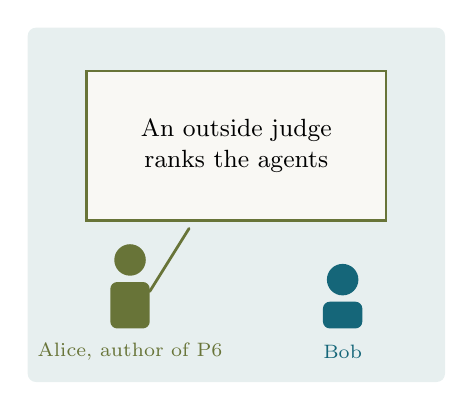
\begin{tikzpicture}[x=1cm,y=1cm]
  \path[use as bounding box] (0,0) rectangle (5.3,4.5);
  \fill[Mist,rounded corners=3pt] (0,0) rectangle (5.3,4.5);
  \draw[Olive,line width=.9pt,fill=Paper] (.75,2.05) rectangle (4.55,3.95);
  \node[font=\small,align=center] at (2.65,3.0) {An outside judge\\ranks the agents};
  \fill[Olive] (1.3,1.55) circle (.2);
  \fill[Olive,rounded corners=2.5pt] (1.05,.68) rectangle (1.55,1.27);
  \draw[Olive,line width=1pt,line cap=round] (1.55,1.15) -- (2.05,1.95);
  \node[font=\scriptsize,text=Olive] at (1.3,.38) {Alice, author of P6};
  \fill[Teal] (4.0,1.3) circle (.2);
  \fill[Teal,rounded corners=2.5pt] (3.75,.68) rectangle (4.25,1.02);
  \node[font=\scriptsize,text=Teal] at (4.0,.38) {Bob};
\end{tikzpicture}
\end{column}
\begin{column}{.67\textwidth}
  \dline{Teal}{Bob}{``Why use a judge? Could you not ask the agents directly?''}
  \dline{Olive}{Alice}{``We could \ldots\ but wouldn't they misreport?''}
  \dline{Teal}{Bob}{``Glad you ask. I have just heard of a mechanism-design paper about that \ldots''}
  \dline{Olive}{Alice}{``Interesting!''}
\end{column}
\end{columns}
\vfill
\paperpair{\Psix}{\Qfour}
% \smallprint{Vincent Danos\quad Elham Kashefi\quad William Waites\hfill github.com/vd1/pathfinder}
\note{Timing: 45 seconds. This is a made-up seminar exchange, not the history of how these papers met.
P6 uses an external AI judge; it does not assume strategic participants report truthfully.
Q4 supplies conditional incentives for truthful reporting. The natural question is whether the latter
can replace the former. Pathfinder tries to systematise both the generation of such questions and
the research that follows them. We will return to what this particular connection actually established.}
\end{frame}

\begin{frame}[t]{What if we asked across an entire collection?}
\kicker{Mechanism design $\times$ agent cooperation}
\begin{columns}[T,onlytextwidth]
\begin{column}{.63\textwidth}
  \resizebox{11.2cm}{!}{\input{assets/2026-09-16-200514/pilot-heatmap.tex}}
\end{column}
\begin{column}{.33\textwidth}
  \vspace{4mm}
  \renewcommand{\arraystretch}{1.25}
  \begin{tabular}{@{}r@{\hspace{4mm}}l@{}}
  {\rmfamily\fontsize{34}{36}\selectfont 100} & possible encounters\\
  {\rmfamily\fontsize{34}{36}\selectfont 14} & investigated pairs\\
  {\rmfamily\fontsize{34}{36}\selectfont\color{Rust} 5} & accepted manuscripts\\
  \end{tabular}\par\vspace{7mm}
  {\small
  \tikz[baseline=-.6ex]{\shade[left color=Paper,right color=Teal] (0,-.11) rectangle (.62,.11);
    \draw[gray!50,line width=.25pt] (0,-.11) rectangle (.62,.11);}\enspace feasibility $\times$ gain\par\vspace{1.5mm}
  \tikz[baseline=-.6ex]{\draw[black,line width=.85pt] (0,-.13) rectangle (.62,.13);}\enspace investigated\par\vspace{1.5mm}
  \makebox[6.2mm][c]{$\star$}\enspace internally accepted}\vspace{3mm}
  % \smallprint{Acceptance is a workflow verdict, not external scientific validation.}
\end{column}
\end{columns}
\vspace{1mm}
% \paperpair{\Qfour}{\Psix}
\note{Timing: 45 seconds. The heatmap is the root 10 by 10 experiment. The scan judges possible
research connections, not textual similarity. Thirteen pairs met the score threshold of 1500;
an already-started pair scoring 600 was retained, giving fourteen investigations. Five manuscripts
were internally accepted. Point out Q4P6, at row four and column six. The Q1P7 zero is the separate
16 September rescan; the original response was unparseable. Selection and acceptance are not an
estimate of a discovery rate, and we have not assessed what alternative selection policies would produce.}
\end{frame}

\begin{frame}[t]{Scan. Research. Edit.}
\vspace{3mm}
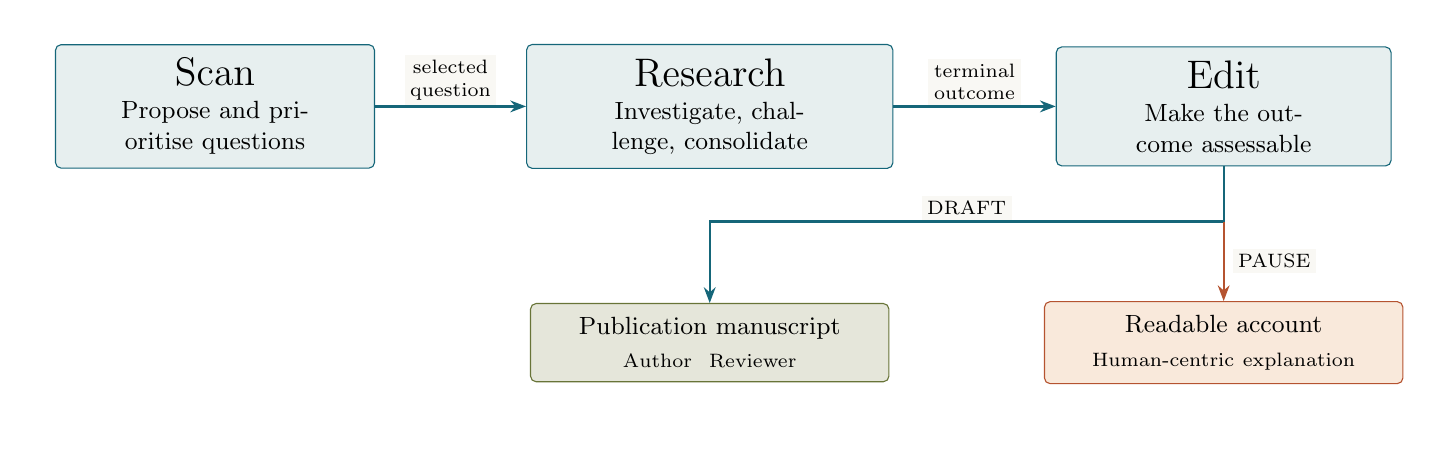
\begin{tikzpicture}[x=1.22cm,y=1cm]
  \path[use as bounding box] (0,-.2) rectangle (14.5,5.0);
  \node[state,text width=3.7cm,minimum height=1.5cm] (scan) at (1.95,4.0)
    {{\Large\rmfamily Scan}\\[1pt]\small Propose and prioritise questions};
  \node[state,text width=4.3cm,minimum height=1.5cm] (research) at (7.1,4.0)
    {{\Large\rmfamily Research}\\[1pt]\small Investigate, challenge, consolidate};
  \node[state,text width=3.9cm,minimum height=1.5cm] (edit) at (12.45,4.0)
    {{\Large\rmfamily Edit}\\[1pt]\small Make the outcome assessable};
  \draw[flow] (scan) -- node[lab,above] {selected\\question} (research);
  \draw[flow] (research) -- node[lab,above] {terminal\\outcome} (edit);
  \node[paused,text width=4.2cm] (account) at (12.45,1.0)
    {Readable account\\[1pt]\scriptsize Human-centric explanation};
  \node[state,fill=Olive!14!Paper,draw=Olive,text width=4.2cm] (paper) at (7.1,1.0)
    {Publication manuscript\\[1pt]\scriptsize Author $\rightleftarrows$ Reviewer};
  \coordinate (editbranch) at ([yshift=-7mm]edit.south);
  \draw[draw=Teal,line width=.8pt] (edit.south) -- (editbranch);
  \draw[flow] (editbranch) -| node[lab,above,pos=.25] {DRAFT} (paper.north);
  \draw[flow,draw=Rust] (editbranch) -- node[lab,right,xshift=1mm] {PAUSE} (account.north);
\end{tikzpicture}
\takeaway{The output may be a result, an obstruction, a mistake in either paper, or an account of what is missing to pursue the connexion.}
\note{Timing: 45 seconds. Explain only the phases, not the formal state notation. Scan generates
the seminar question. Research tests it and can reformulate it. Both DRAFT and PAUSE outcomes enter
editing. The diagram shows their main destinations: a publication manuscript for DRAFT, a readable
human-centric account for PAUSE, including capped pauses. The implementation also permits a readable
account after DRAFT; the diagram emphasises the manuscript route for that outcome. Editing is not
another research pass. Successful manuscript review and a successful build are both
required for acceptance. The agent-facing specification and conformance tests are in the paper.}
\end{frame}

\begin{frame}[t]{The research phase}
% \kicker{Shared evidence; independent verification; bounded loops}
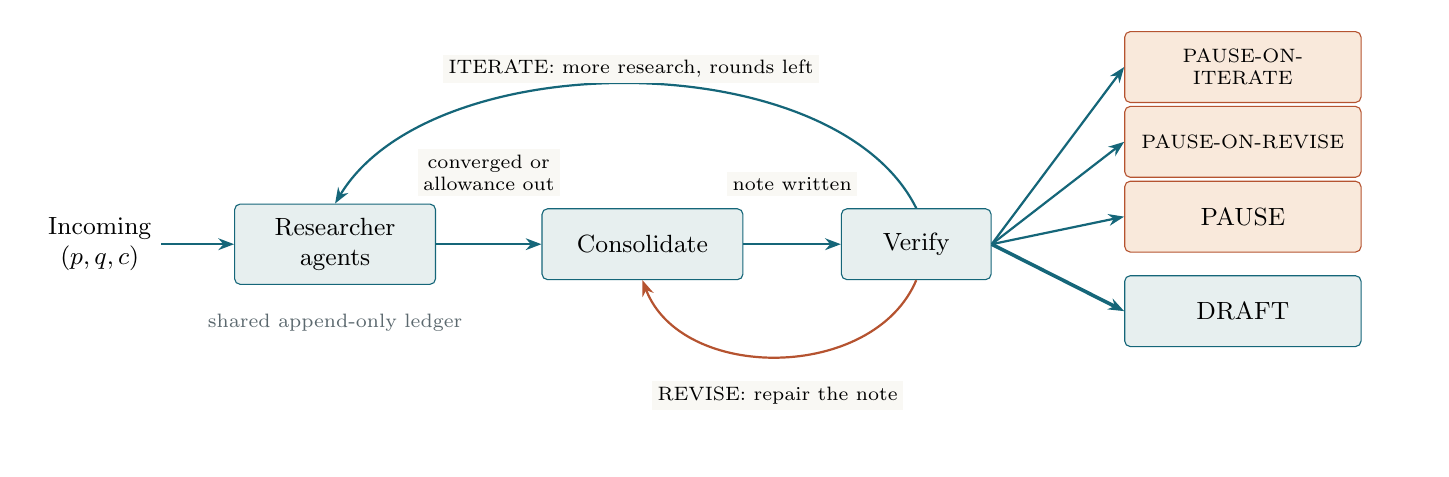
\begin{tikzpicture}[x=1.22cm,y=1cm]
  \path[use as bounding box] (0,-.8) rectangle (14.5,4.55);
  \node[font=\small,align=center] (incoming) at (.75,1.8) {Incoming\\$(p,q,c)$};
  \node[state,text width=2.2cm] (agents) at (3.2,1.8) {Researcher\\agents};
  \node[state,text width=2.2cm] (conso) at (6.4,1.8) {Consolidate};
  \node[state,text width=1.55cm] (verify) at (9.25,1.8) {Verify};
  \node[paused,text width=2.65cm,font=\scriptsize] (poi) at (12.65,4.05) {PAUSE-ON-ITERATE};
  \node[paused,text width=2.65cm,font=\scriptsize] (por) at (12.65,3.1) {PAUSE-ON-REVISE};
  \node[paused,text width=2.65cm,font=\small] (pause) at (12.65,2.15) {PAUSE};
  \node[state,text width=2.65cm] (draft) at (12.65,.95) {DRAFT};
  \draw[flow] (incoming) -- (agents);
  \draw[flow] (agents) -- node[lab,above,yshift=6mm] {converged or\\allowance out} (conso);
  \draw[flow] (conso) -- node[lab,above,yshift=6mm] {note written} (verify);
  \draw[flow] (verify.north) .. controls (8.4,4.35) and (4.2,4.35) ..
    node[lab,above] {ITERATE: more research, rounds left} (agents.north);
  \draw[flow,draw=Rust] (verify.south) .. controls (8.8,.05) and (6.8,.05) ..
    node[lab,below,yshift=-3mm] {REVISE: repair the note} (conso.south);
  \draw[flow] (verify.east) -- (poi.west);
  \draw[flow] (verify.east) -- (por.west);
  \draw[flow] (verify.east) -- (pause.west);
  \draw[flow,line width=1.3pt] (verify.east) -- (draft.west);
  \node[font=\scriptsize,text=Muted,align=center] at (3.2,.8) {shared append-only ledger};
  % \node[font=\scriptsize,text=Muted,anchor=west] at (.2,-.6)
  %   {$c$: optional seed connection. Empty research can also end in PAUSE; omitted here for clarity.};
\end{tikzpicture}
\takeaway{Research question changes after iterations.\\ Seed $c$ is a hypothesis to investigate, not a claim the agents must pursue.\\ Agents are
resource-bound.}
\note{Timing: 1 minute. The researchers share an append-only ledger and can disagree.
Their readiness is invalidated by subsequent substantive work. The consolidation is reviewed by a
fresh verifier. Iterate means more research; revise means repair the note. The revise arc is below
the note-written arc. A pause-on-iterate records an exhausted iteration allowance, not necessarily
a dead end. We have discussed adding a separate scientific assessment, PAUSE-PLUS versus PAUSE-MINUS;
that is a proposed refinement, not an implemented state transition in this diagram.}
\end{frame}

\begin{frame}[t]{Practicalities}
\vspace{4mm}
\begin{columns}[T,onlytextwidth]
  \begin{column}{.3\textwidth}
    {\Large\color{Teal}\textbf{Nothing is lost}}\par\vspace{3mm}
    Every step is saved as it happens.\par\vspace{2mm}
    After a crash, work resumes where it stopped.
  \end{column}
  \begin{column}{.3\textwidth}
    {\Large\color{Teal}\textbf{Spending is bounded}}\par\vspace{3mm}
    Every call records its time and its cost.\par\vspace{2mm}
    Each loop has a limit, and the budget is checked before new work starts.
  \end{column}
  \begin{column}{.3\textwidth}
    {\Large\color{Teal}\textbf{Reading is reused}}\par\vspace{3mm}
    Every call starts with the same material.\par\vspace{2mm}
    What the model has already read costs much less to read again.
  \end{column}
\end{columns}
\vspace{9mm}
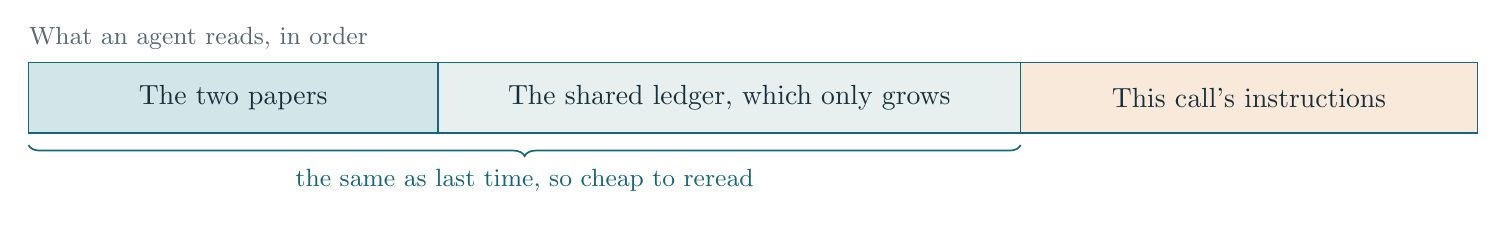
\begin{tikzpicture}[x=1cm,y=1cm]
  \node[anchor=west,text=Muted,font=\small,inner sep=0pt]
    at (0,1.2) {What an agent reads, in order};
  \fill[CardFill] (0,0) rectangle (5.2,.9);
  \fill[Mist] (5.2,0) rectangle (12.6,.9);
  \fill[Warm] (12.6,0) rectangle (18.4,.9);
  \draw[Teal,line width=.6pt] (0,0) rectangle (18.4,.9);
  \draw[Teal,line width=.6pt] (5.2,0) -- (5.2,.9) (12.6,0) -- (12.6,.9);
  \node[text=Ink] at (2.6,.45) {The two papers};
  \node[text=Ink] at (8.9,.45) {The shared ledger, which only grows};
  \node[text=Ink] at (15.5,.45) {This call's instructions};
  \draw[decorate,decoration={brace,mirror,amplitude=4pt},Teal,line width=.6pt] (0,-.15) -- (12.6,-.15)
    node[midway,below=5pt,font=\small,text=Teal] {the same as last time, so cheap to reread};
\end{tikzpicture}
\takeaway{Machinery keeps the work safe and the bill predictable}
\note{Timing: 45 seconds. These are operational mechanisms, not additional scientific verdicts.
The runner keeps artifacts, a shared ledger and stage state. Recovery resumes from a recorded
boundary; it does not promise to recover an interrupted model's internal state or avoid every
duplicate call. Transport failure and unreadable output are handled separately from a scientific
pause, with bounded retries and explicit intervention where needed. Receipts track call-level
tokens and time; the older pilot lacked complete cache counters, as the economics slide explains.
Budget admission uses available accounting and estimates, and in-flight work can exceed that estimate.
For calls using inline context, common paper text comes first, then the growing ledger, then
call-specific instructions. Prefix reuse depends on provider cache behaviour; it is not guaranteed.
Researchers also read new ledger entries before changing direction or declaring ready.}
\end{frame}

\begin{frame}[t]{Q4P6: when can we dispense with the judge?}
\paperpair{\Qfour}{\Psix}
\vspace{1mm}
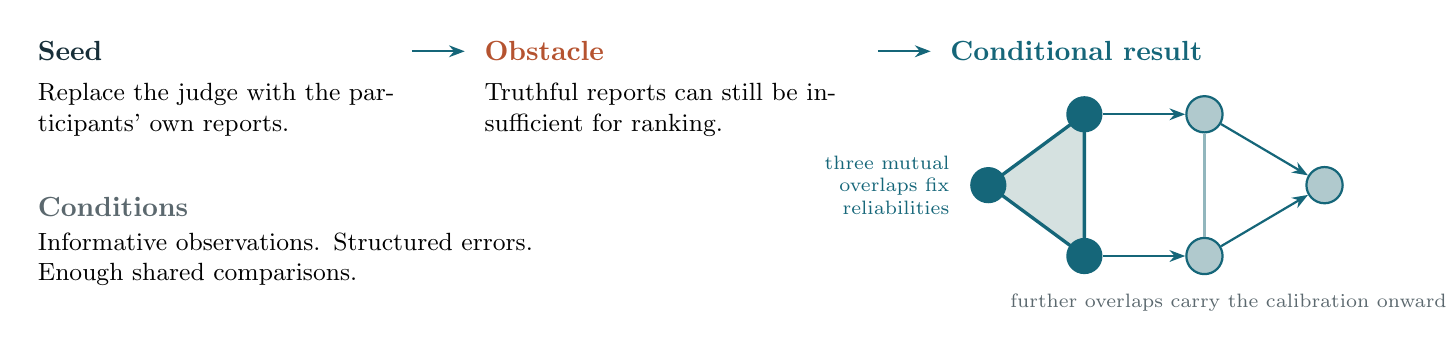
\begin{tikzpicture}[x=1.22cm,y=1cm]
  \path[use as bounding box] (0,-.3) rectangle (14.5,3.5);
  \node[anchor=west,inner sep=0pt] at (.1,3.2) {\stage[Ink]{Seed}};
  \node[anchor=west,inner sep=0pt] at (4.75,3.2) {\stage[Rust]{Obstacle}};
  \node[anchor=west,inner sep=0pt] at (9.6,3.2) {\stage{Conditional result}};
  \node[align=left,text width=4.6cm,anchor=north west,font=\small,inner sep=0pt] at (.1,2.8)
    {Replace the judge with the participants' own reports.};
  \node[align=left,text width=4.8cm,anchor=north west,font=\small,inner sep=0pt] at (4.75,2.8)
    {Truthful reports can still be insufficient for ranking.};
  \draw[flow] (4.0,3.2) -- (4.55,3.2);
  \draw[flow] (8.85,3.2) -- (9.4,3.2);
  % observers are dots; an edge joins two observers who judged the same comparison.
  % A triangle of mutual overlaps fixes three reliabilities; further overlaps carry the calibration onward.
  \coordinate (a) at (10.0,1.5); \coordinate (b) at (11.0,2.4); \coordinate (c) at (11.0,.6);
  \fill[Teal!16!Paper] (a) -- (b) -- (c) -- cycle;
  \draw[Teal,line width=1.2pt,line join=round] (a) -- (b) -- (c) -- cycle;
  \node[agent,minimum size=4.6mm] (na) at (a) {};
  \node[agent,minimum size=4.6mm] (nb) at (b) {};
  \node[agent,minimum size=4.6mm] (nc) at (c) {};
  \node[agent,minimum size=4.6mm,fill=Teal!32!Paper,draw=Teal,line width=.8pt] (nd) at (12.25,2.4) {};
  \node[agent,minimum size=4.6mm,fill=Teal!32!Paper,draw=Teal,line width=.8pt] (ne) at (12.25,.6) {};
  \node[agent,minimum size=4.6mm,fill=Teal!32!Paper,draw=Teal,line width=.8pt] (nf) at (13.5,1.5) {};
  \draw[Teal!45!Paper,line width=.8pt] (nd) -- (ne);
  \draw[flow] (nb) -- (nd); \draw[flow] (nc) -- (ne);
  \draw[flow] (nd) -- (nf); \draw[flow] (ne) -- (nf);
  \node[font=\scriptsize,align=right,anchor=east,text=Teal,inner sep=0pt] at (9.6,1.5) {three mutual\\overlaps fix\\reliabilities};
  \node[font=\scriptsize,align=center,anchor=north,text=Muted,inner sep=0pt] at (12.5,.12) {further overlaps carry the calibration onward};
  \node[anchor=north west,inner sep=0pt] at (.1,1.35) {\stage[Muted]{Conditions}};
  \node[anchor=north west,text width=9.6cm,font=\small,align=left,inner sep=0pt] at (.1,.9)
    {Informative observations. Structured errors.\\Enough shared comparisons.};
\end{tikzpicture}
\takeaway{\textbf{Under these conditions, peer reports identify the model's ranking without an external judge.}}
\vspace{1mm}\smallprint{Population-level, conditional application. A model-defined ranking is not automatically causal contribution.}
\note{Timing: 1 minute 45 seconds. Q4 addresses incentives, not whether the reports contain enough information
to rank contributions. Under stable symmetric errors, observers that are better than chance,
and conditional independence on a shared comparison, overlaps let us identify their reliabilities.
A calibration triangle anchors this, and connectivity propagates it. A connected comparison graph
then identifies the Bradley--Terry ranking up to an additive constant. This uses established
single-coin calibration ideas, not a new general calibration theorem. The truthful-report mechanism
still needs its own belief assumptions. The result is a conditional no-judge variation on P6,
not a correction to a paper that already relied on strategic user reports.}
\end{frame}

\begin{frame}[t]{Q7P1: a tale of two runs}
\paperpair{\Qseven}{\Pone}
{\small\textbf{Shared seed:} adapt resource sharing to participants who care about bad outcomes.}\par\vspace{2mm}
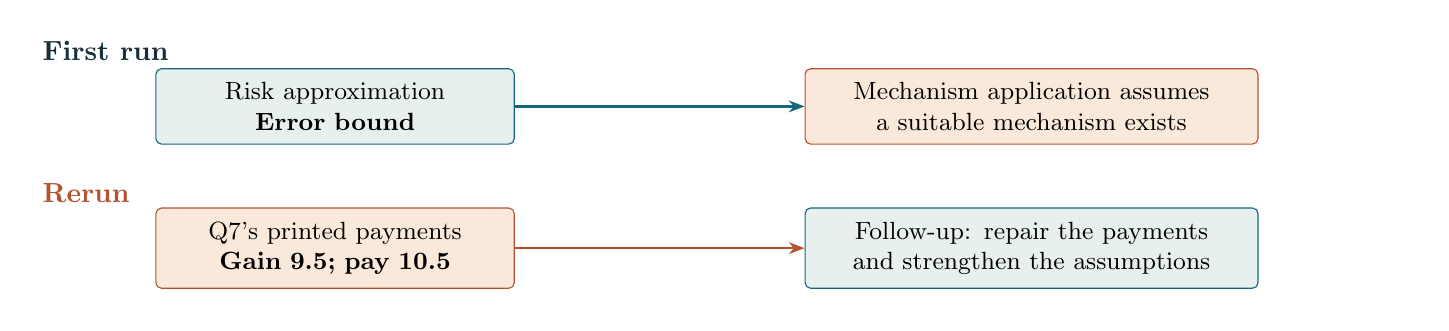
\begin{tikzpicture}[x=1.22cm,y=1cm]
  \path[use as bounding box] (0,-.25) rectangle (14.5,3.25);
  \node[anchor=west,inner sep=0pt] at (.15,2.95) {\stage[Ink]{First run}};
  \node[state,text width=4.2cm] (bound) at (3.2,2.25) {Risk approximation\\\textbf{Error bound}};
  \node[paused,text width=5.4cm] (premise) at (10.45,2.25)
    {Mechanism application assumes\\a suitable mechanism exists};
  \draw[flow] (bound) -- (premise);
  \node[anchor=west,inner sep=0pt] at (.15,1.15) {\stage[Rust]{Rerun}};
  \node[paused,text width=4.2cm] (audit) at (3.2,.45) {Q7's printed payments\\\textbf{Gain 9.5; pay 10.5}};
  \node[state,text width=5.4cm] (repair) at (10.45,.45)
    {Follow-up: repair the payments\\and strengthen the assumptions};
  \draw[flow,draw=Rust] (audit) -- (repair);
\end{tikzpicture}\par\vspace{1mm}
{\small The first run bounded the error in estimating risk, but left the resource-sharing rules conditional.
The rerun found that Q7 could charge a participant more than they gained, prompting a repair under stronger assumptions.}\par\vspace{2mm}
\takeaway{\textbf{The approximation bound survives. Its intended application needed repair.}}
\note{Timing: 1 minute 45 seconds. The first paper establishes error control for an expected empirical,
smoothed risk approximation, and near-optimal true-risk choices over the same feasible set.
Its mechanism application is conditional. The independent rerun finds incompatible conditions
and a failure of the printed payment rule in Q7, not P1. In an equilibrium example, a participant
gets benefit 9.5 and pays 10.5. This does not refute a conditional theorem whose premises fail;
it shows that the printed construction cannot support the desired application. A subsequent
paper follow-up adds an opponent-only payment term and stronger curvature and feasibility assumptions.
It proves guarantees for a fixed surrogate, with error control relative to true risk. The old
approximation bound survives because it did not depend on those payments. Efficient learning in
practice remains open. These are two runs, not a single uninterrupted chain of reasoning.}
\end{frame}

\begin{frame}[t]{Q3P3: a promising question, an unfinished test}
\paperpair{\Qthree}{\Pthree}
\vspace{2mm}
\begin{columns}[T,onlytextwidth]
  \begin{column}{.315\textwidth}
    \stage[Ink]{Seed: spot a rush to finish}\par\vspace{2mm}
    \small Q3 finds urgency in traders' language just before a trade.
    P3's reviewers sometimes agree too soon.\par\vspace{2mm}
    \textbf{Could Q3's language analysis warn when P3's reviewers are rushing to agree?}
  \end{column}
  \begin{column}{.315\textwidth}
    \stage{Shift: test simpler agents}\par\vspace{2mm}
    \small The researchers found that simple random traders could do well under Q3's rules.\par\vspace{2mm}
    This suggested a different question for P3:
    \textbf{does the critic help, or do extra rounds of review explain the gain?}
  \end{column}
  \begin{column}{.315\textwidth}
    \stage[Rust]{Test: compare fairly}\par\vspace{2mm}
    \small Compare a reviewer working alone with a reviewer helped by a critic.\par\vspace{2mm}
    Let both review and repair repeatedly, on the same tasks, with equal computing budgets.\par\vspace{2mm}
    \textbf{The required materials were unavailable.}
  \end{column}
\end{columns}
\takeaway{Q3 inspired the test; it did not establish the answer for P3. Neither the seed nor the revised connexion was demonstrated.}
\vspace{1mm}\smallprint{Original outcome: PAUSE-ON-ITERATE. Missing evidence, not proof that the critic is ineffective.}
\note{Timing: 1 minute 30 seconds. The original seed transfers Q3's analysis of traders' language
to P3's premature reviewer--critic agreement. Urgency before a trade is not itself evidence of
premature agreement in code review; that proposed connection was not established.
The researchers then changed direction. Their constrained random-trader benchmark performed well
under Q3's stated market rules, conditional on the LLM traders complying with the same constraints.
This motivated separating the value of agents' information from the rules governing their interaction.
On the P3 side, some baselines
revise once, while adversarial review and another stronger method revisit revised work. The proposed
control compares repeated single review and adversarial review with equal resources, plus a random
critic matched to disagreement rates. The supplied record lacked the tasks, execution setup and
access needed to reproduce and extend the reported experiments. A new benchmark would test a related
hypothesis, not explain those results. The first thread exhausted its iteration cap. A further
continuation was requested, but no completed new outcome was available when these slides were built.}
\end{frame}

\begin{frame}[t]{Breadth is cheap. Investigation dominates.}
\kicker{Economics of the 10$\times$10 pilot}
\begin{columns}[T,onlytextwidth]
\begin{column}{.58\textwidth}
{\rmfamily\fontsize{30}{34}\selectfont \$\ScenarioTotal}\quad\small recorded-token scenario\par
\vspace{3mm}
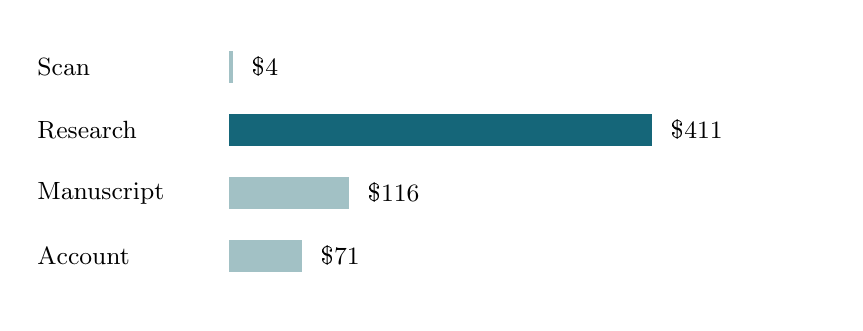
\begin{tikzpicture}[x=1.22cm,y=1cm]
  \path[use as bounding box] (0,-.3) rectangle (8.4,3.2);
  \foreach \label/\value/\y in {Scan/3.74692/2.7,Research/410.56226/1.9,Manuscript/116.11062/1.1,Account/70.52111/.3}{
    \pgfmathsetmacro{\barw}{4.4*\value/410.56226}
    \node[anchor=west,font=\small] at (0,\y) {\label};
    \pgfmathparse{\value>400 ? 100 : 38}\edef\barshade{\pgfmathresult}
    \fill[Teal!\barshade!Paper] (2.1,\y-.2) rectangle (2.1+\barw,\y+.2);
    \node[anchor=west,font=\small] at (2.2+\barw,\y)
      {\$\pgfmathprintnumber[fixed,precision=0]{\value}};
  }
\end{tikzpicture}
\smallprint{\RecordedInput M recorded input tokens; \RecordedOutput M output.\\
Flat GPT-6 Standard rates: \$10/M input, \$50/M output.}
\end{column}
\begin{column}{.39\textwidth}
{\rmfamily\fontsize{26}{29}\selectfont \CampaignSpan\,h}\quad campaign span\par
\smallprint{Includes pauses and owner continuations.}\vspace{3mm}
{\rmfamily\fontsize{26}{29}\selectfont \AgentHours\,h}\quad summed call time\par
\smallprint{Overlapping calls; not wall-clock duration.}\vspace{3mm}
{\rmfamily\fontsize{26}{29}\selectfont 25\,h}\quad illustrative human scan\par
\smallprint{Assuming 15 minutes per pair.\\Not a measured human control.}
\end{column}
\end{columns}
\vspace{2mm}
\takeaway{\textbf{Scenario, not a bill:} cache usage was incompletely logged; exact repricing is unavailable.}
\vspace{1mm}\smallprint{Common tariff, not an observed medium-effort run. Subscription quota is separate.
\href{https://developers.openai.com/api/docs/models/gpt-6-astra}{OpenAI pricing, 16 September 2026}.}
\note{Timing: 1 minute. All displayed model dollar figures use the same GPT-6 Standard
short-context tariff on the input and output tokens actually recorded. This deliberately simple
scenario treats recorded input as uncached and omits unrecorded cache usage. Historical Claude
cache reads and writes were not retained; Codex cached shares are also missing. Long-context
adjustments and separately billed tools cannot be reconstructed. Thus 601 dollars is neither a
measured GPT-6 bill nor a reliable upper or lower bound on one. It is a transparent illustration
of pricing the available token counters. The 330 calls span 43.7 hours but sum to 8.1 agent-hours.
Neither number establishes a human speedup. The human scan estimate assumes 15 minutes for each
of 100 pairs, and is not matched for quality. Choosing medium effort does not predict token use.}
\end{frame}

\begin{frame}[t]{Scale-up: the Julien Michel validation experiment}
\kicker{Quantum methods for computational chemistry}
\begin{columns}[T,onlytextwidth]
\begin{column}{.52\textwidth}
  \centering
  {\setlength{\fboxsep}{3pt}\setlength{\fboxrule}{.5pt}\fcolorbox{Mist}{white}{%
  
\includegraphics[width=\dimexpr\linewidth-7pt\relax,height=7.05cm,keepaspectratio]{\assetdir/julien-dashboard.png}}}
\end{column}
\begin{column}{.45\textwidth}
  {\rmfamily\fontsize{30}{33}\selectfont 71$\times$82}\par
  5,822 scored pairs\par\vspace{4mm}
  {\small \textbf{59} pairs selected for research\par\vspace{2mm}
  \textbf{98} finished threads
  % \par\vspace{1mm}
  (51 PAUSE, 44 CONTINUE)\par\vspace{2mm}
  \textbf{3} DRAFT outcomes}\par\vspace{2mm}
  {\small\color{Teal}\textbf{One pair can suggest several connexions.}}\par\vspace{2mm}
  % \smallprint{DRAFT is an internal research outcome, not external validation.}\vspace{4mm}
  {\small The expert already knows\\one side of the connexion.}\par\vspace{2mm}
  \smallprint{Expert assessment becomes a search for directions in their own programme.}
\end{column}
\end{columns}
\vspace{2mm}
% \takeaway{\textbf{Human validation:} do the notes add something new and useful to the expert's research?}
% \smallprint{Darker cells indicate higher scan scores, scientific quality as scored by Opus 5.}
\note{Timing: 1 minute. The admitted release has 82 papers on each side; the original
working inventories contain additional excluded rows. The supplied dashboard screenshot replaces
the earlier reconstructed heatmap. Its legend marks selection for Phase E and DRAFT outcomes.
Do not attach the old single-instrument coverage figures or snapshot date to this screenshot.
Selection and DRAFT are workflow outcomes, not independent scientific validation.
This is a different corpus and protocol from the 10 by 10 pilot. The expert's familiarity
with one side makes evaluating candidate connections less costly and more directly relevant.
The 59 selected pairs and 98 finished E-prime threads count different units. The thread outcomes
are 51 paused, 44 continue and 3 draft-ready. CONTINUE ends a run, not the research question.
A pair can suggest several connexions, and an investigation can also have follow-up rounds.
The 98-thread count is not a count of distinct connexions or terminal research outcomes.
Human validation asks whether a note changes what an expert understands or would investigate next:
is the connection already familiar, are its assumptions meaningful, and does its conclusion help?
This is an evaluation question, not a claim that the reported notes have passed that evaluation.
Expert judgement complements proofs and experiments; it does not replace them.
A supported obstruction can be useful even when the research ends at PAUSE rather than DRAFT.}
\end{frame}

\begin{frame}[t]{Scale-up in quantum: QSL meets vendor applications}
% \kicker{The companion paper's frozen experiment}
\begin{columns}[T,onlytextwidth]
\begin{column}{.62\textwidth}
  {\small \QSLColumns\ vendor-side paper artefacts (columns)}\par\vspace{2mm}
  {\setlength{\fboxsep}{3pt}\setlength{\fboxrule}{.5pt}\fcolorbox{Mist}{white}{%
  
\includegraphics[width=11.0cm,height=6.7cm,keepaspectratio]{\assetdir/qsl-dashboard.pdf}}}
  % \smallprint{\QSLRows\ QSL papers (rows). Frozen paper-pair universe.}
\end{column}
\begin{column}{.35\textwidth}
  {\rmfamily\fontsize{30}{33}\selectfont \QSLRows$\times$\QSLColumns}\par
  \QSLPairs\ candidate pairs\par\vspace{2.5mm}
  {\small \textbf{100} pairs in the original selection}\par\vspace{2mm}
  {\small Fully scored by two judges (Opus 5 and gpt-5.6).\\Global rank correlation: \textbf{0.740}.}\par\vspace{2mm}
  \begin{columns}[T,onlytextwidth]
    \begin{column}{.23\linewidth}
\includegraphics[width=\linewidth]{\assetdir/qsl-paper.png}\end{column}
    \begin{column}{.72\linewidth}{\fontsize{8.5}{11}\selectfont\rmfamily
      Pathfinder: hypothesis generation across the quantum software-hardware boundary}\par
      \vspace{1mm}\smallprint{Danos, Kashefi, Waites\\Companion manuscript, 2026}
    \end{column}
  \end{columns}
  \vspace{1.5mm}
  {\small\color{Teal}\textbf{Later E-prime campaign}}\par\vspace{1mm}
  {\small \textbf{147} final notes (144 PAUSE, \textbf{3 DRAFT})}\par
  \smallprint{Expanded campaign, not just the original 100 pairs.\\Watchboard snapshot: 14 September, 20:42 UTC.}
\end{column}
\end{columns}
\vspace{2mm}
%\takeaway{A method, proof or test on one side can challenge a platform claim on the other.}
% \smallprint{Shown: Opus 5, technical hook $\times$ interest. Frozen 88$\times$124 corpus; later inventory growth is not this experiment.}
\note{Timing: 1 minute. Use the companion manuscript's frozen 88 by 124 universe,
not the approximate 150 by 150 live-corpus ambition. Both Opus 5 and GPT-5.6 Sol scored 10912 pairs.
The heatmap displays Opus scores; its scale differs from the pilot's feasibility and gain axes.
The paper reports global Spearman correlation 0.740 but only 12--36 overlap between exact
top-100 lists when cutoff ties are resolved. Thus broad rank agreement does not mean agreement
about the best candidates. The paper audits selected candidate experiments; it does not report
their execution or a measured discovery rate. Source: the local companion manuscript and its
frozen-corpus ledger.}
\end{frame}

\begin{frame}[plain]
\vspace{12mm}
{\rmfamily\fontsize{36}{42}\selectfont Questions}\par
\vspace{5mm}{\color{Teal}\rule{28mm}{1.5pt}}\par\vspace{8mm}
{\color{Muted}How much of creativity is connexion?}\par
{\color{Muted}What is the density $d(Q,P)$ of $Q\times P$ in good ideas?}\par
{\color{Muted}Can agents also help choose which corpora to bring together?}\par
{\color{Muted}How to trade-off search space restriction and loss rate?}\par
\vspace{6mm}
{\large If agents can make the connexions and also \\ investigate what follows \ldots}\par\vspace{6mm}
{\large What are the other things humans do in science?}\par\vspace{3mm}
{\rmfamily\fontsize{15}{21}\selectfont\color{Teal}
Choosing questions.\quad Inventing concepts.\\Judging significance.\quad Applying for funding.}\par
\vspace{8mm}


\begin{tikzpicture}[remember picture,overlay]
  \begin{scope}[shift={([xshift=-48mm,yshift=-10mm]current page.east)},x=3.6mm,y=3.6mm,opacity=.5]
    % generated by build_title_grid.py from pilot-heatmap.tex; do not edit
\fill[Teal!59!Paper,rounded corners=.5pt] (0.07,-0.93) rectangle (0.93,-0.07);
\draw[Ink,line width=.7pt,rounded corners=.5pt] (0.07,-0.93) rectangle (0.93,-0.07);
\fill[Teal!25!Paper,rounded corners=.5pt] (1.07,-0.93) rectangle (1.93,-0.07);
\draw[Ink,line width=.7pt,rounded corners=.5pt] (1.07,-0.93) rectangle (1.93,-0.07);
\fill[Rust] (1.50,-0.50) circle (.17);
\fill[Teal!17!Paper,rounded corners=.5pt] (2.07,-0.93) rectangle (2.93,-0.07);
\fill[Teal!14!Paper,rounded corners=.5pt] (3.07,-0.93) rectangle (3.93,-0.07);
\fill[Teal!12!Paper,rounded corners=.5pt] (4.07,-0.93) rectangle (4.93,-0.07);
\fill[Teal!48!Paper,rounded corners=.5pt] (5.07,-0.93) rectangle (5.93,-0.07);
\draw[Ink,line width=.7pt,rounded corners=.5pt] (5.07,-0.93) rectangle (5.93,-0.07);
\fill[Rust] (5.50,-0.50) circle (.17);
\fill[Ink!6!Paper,rounded corners=.5pt] (6.07,-0.93) rectangle (6.93,-0.07);
\fill[Teal!12!Paper,rounded corners=.5pt] (7.07,-0.93) rectangle (7.93,-0.07);
\fill[Teal!36!Paper,rounded corners=.5pt] (8.07,-0.93) rectangle (8.93,-0.07);
\fill[Teal!45!Paper,rounded corners=.5pt] (9.07,-0.93) rectangle (9.93,-0.07);
\fill[Ink!6!Paper,rounded corners=.5pt] (0.07,-1.93) rectangle (0.93,-1.07);
\fill[Ink!6!Paper,rounded corners=.5pt] (1.07,-1.93) rectangle (1.93,-1.07);
\fill[Ink!6!Paper,rounded corners=.5pt] (2.07,-1.93) rectangle (2.93,-1.07);
\fill[Ink!6!Paper,rounded corners=.5pt] (3.07,-1.93) rectangle (3.93,-1.07);
\fill[Ink!6!Paper,rounded corners=.5pt] (4.07,-1.93) rectangle (4.93,-1.07);
\fill[Ink!6!Paper,rounded corners=.5pt] (5.07,-1.93) rectangle (5.93,-1.07);
\fill[Ink!6!Paper,rounded corners=.5pt] (6.07,-1.93) rectangle (6.93,-1.07);
\fill[Ink!6!Paper,rounded corners=.5pt] (7.07,-1.93) rectangle (7.93,-1.07);
\fill[Teal!17!Paper,rounded corners=.5pt] (8.07,-1.93) rectangle (8.93,-1.07);
\fill[Ink!6!Paper,rounded corners=.5pt] (9.07,-1.93) rectangle (9.93,-1.07);
\fill[Teal!15!Paper,rounded corners=.5pt] (0.07,-2.93) rectangle (0.93,-2.07);
\fill[Ink!6!Paper,rounded corners=.5pt] (1.07,-2.93) rectangle (1.93,-2.07);
\fill[Teal!59!Paper,rounded corners=.5pt] (2.07,-2.93) rectangle (2.93,-2.07);
\draw[Ink,line width=.7pt,rounded corners=.5pt] (2.07,-2.93) rectangle (2.93,-2.07);
\fill[Ink!6!Paper,rounded corners=.5pt] (3.07,-2.93) rectangle (3.93,-2.07);
\fill[Teal!12!Paper,rounded corners=.5pt] (4.07,-2.93) rectangle (4.93,-2.07);
\fill[Teal!50!Paper,rounded corners=.5pt] (5.07,-2.93) rectangle (5.93,-2.07);
\draw[Ink,line width=.7pt,rounded corners=.5pt] (5.07,-2.93) rectangle (5.93,-2.07);
\fill[Ink!6!Paper,rounded corners=.5pt] (6.07,-2.93) rectangle (6.93,-2.07);
\fill[Ink!6!Paper,rounded corners=.5pt] (7.07,-2.93) rectangle (7.93,-2.07);
\fill[Teal!93!Paper,rounded corners=.5pt] (8.07,-2.93) rectangle (8.93,-2.07);
\draw[Ink,line width=.7pt,rounded corners=.5pt] (8.07,-2.93) rectangle (8.93,-2.07);
\fill[Teal!86!Paper,rounded corners=.5pt] (9.07,-2.93) rectangle (9.93,-2.07);
\draw[Ink,line width=.7pt,rounded corners=.5pt] (9.07,-2.93) rectangle (9.93,-2.07);
\fill[Teal!17!Paper,rounded corners=.5pt] (0.07,-3.93) rectangle (0.93,-3.07);
\fill[Ink!6!Paper,rounded corners=.5pt] (1.07,-3.93) rectangle (1.93,-3.07);
\fill[Teal!63!Paper,rounded corners=.5pt] (2.07,-3.93) rectangle (2.93,-3.07);
\draw[Ink,line width=.7pt,rounded corners=.5pt] (2.07,-3.93) rectangle (2.93,-3.07);
\fill[Ink!6!Paper,rounded corners=.5pt] (3.07,-3.93) rectangle (3.93,-3.07);
\fill[Teal!11!Paper,rounded corners=.5pt] (4.07,-3.93) rectangle (4.93,-3.07);
\fill[Teal!89!Paper,rounded corners=.5pt] (5.07,-3.93) rectangle (5.93,-3.07);
\draw[Ink,line width=.7pt,rounded corners=.5pt] (5.07,-3.93) rectangle (5.93,-3.07);
\fill[Rust] (5.50,-3.50) circle (.17);
\fill[Ink!6!Paper,rounded corners=.5pt] (6.07,-3.93) rectangle (6.93,-3.07);
\fill[Teal!11!Paper,rounded corners=.5pt] (7.07,-3.93) rectangle (7.93,-3.07);
\fill[Teal!55!Paper,rounded corners=.5pt] (8.07,-3.93) rectangle (8.93,-3.07);
\draw[Ink,line width=.7pt,rounded corners=.5pt] (8.07,-3.93) rectangle (8.93,-3.07);
\fill[Teal!100!Paper,rounded corners=.5pt] (9.07,-3.93) rectangle (9.93,-3.07);
\draw[Ink,line width=.7pt,rounded corners=.5pt] (9.07,-3.93) rectangle (9.93,-3.07);
\fill[Teal!12!Paper,rounded corners=.5pt] (0.07,-4.93) rectangle (0.93,-4.07);
\fill[Ink!6!Paper,rounded corners=.5pt] (1.07,-4.93) rectangle (1.93,-4.07);
\fill[Ink!6!Paper,rounded corners=.5pt] (2.07,-4.93) rectangle (2.93,-4.07);
\fill[Ink!6!Paper,rounded corners=.5pt] (3.07,-4.93) rectangle (3.93,-4.07);
\fill[Ink!6!Paper,rounded corners=.5pt] (4.07,-4.93) rectangle (4.93,-4.07);
\fill[Ink!6!Paper,rounded corners=.5pt] (5.07,-4.93) rectangle (5.93,-4.07);
\fill[Ink!6!Paper,rounded corners=.5pt] (6.07,-4.93) rectangle (6.93,-4.07);
\fill[Ink!6!Paper,rounded corners=.5pt] (7.07,-4.93) rectangle (7.93,-4.07);
\fill[Ink!6!Paper,rounded corners=.5pt] (8.07,-4.93) rectangle (8.93,-4.07);
\fill[Ink!6!Paper,rounded corners=.5pt] (9.07,-4.93) rectangle (9.93,-4.07);
\fill[Teal!11!Paper,rounded corners=.5pt] (0.07,-5.93) rectangle (0.93,-5.07);
\fill[Ink!6!Paper,rounded corners=.5pt] (1.07,-5.93) rectangle (1.93,-5.07);
\fill[Ink!6!Paper,rounded corners=.5pt] (2.07,-5.93) rectangle (2.93,-5.07);
\fill[Ink!6!Paper,rounded corners=.5pt] (3.07,-5.93) rectangle (3.93,-5.07);
\fill[Teal!13!Paper,rounded corners=.5pt] (4.07,-5.93) rectangle (4.93,-5.07);
\fill[Teal!11!Paper,rounded corners=.5pt] (5.07,-5.93) rectangle (5.93,-5.07);
\fill[Ink!6!Paper,rounded corners=.5pt] (6.07,-5.93) rectangle (6.93,-5.07);
\fill[Ink!6!Paper,rounded corners=.5pt] (7.07,-5.93) rectangle (7.93,-5.07);
\fill[Teal!25!Paper,rounded corners=.5pt] (8.07,-5.93) rectangle (8.93,-5.07);
\fill[Teal!16!Paper,rounded corners=.5pt] (9.07,-5.93) rectangle (9.93,-5.07);
\fill[Teal!66!Paper,rounded corners=.5pt] (0.07,-6.93) rectangle (0.93,-6.07);
\draw[Ink,line width=.7pt,rounded corners=.5pt] (0.07,-6.93) rectangle (0.93,-6.07);
\fill[Rust] (0.50,-6.50) circle (.17);
\fill[Ink!6!Paper,rounded corners=.5pt] (1.07,-6.93) rectangle (1.93,-6.07);
\fill[Ink!6!Paper,rounded corners=.5pt] (2.07,-6.93) rectangle (2.93,-6.07);
\fill[Teal!13!Paper,rounded corners=.5pt] (3.07,-6.93) rectangle (3.93,-6.07);
\fill[Teal!12!Paper,rounded corners=.5pt] (4.07,-6.93) rectangle (4.93,-6.07);
\fill[Teal!14!Paper,rounded corners=.5pt] (5.07,-6.93) rectangle (5.93,-6.07);
\fill[Teal!51!Paper,rounded corners=.5pt] (6.07,-6.93) rectangle (6.93,-6.07);
\draw[Ink,line width=.7pt,rounded corners=.5pt] (6.07,-6.93) rectangle (6.93,-6.07);
\fill[Rust] (6.50,-6.50) circle (.17);
\fill[Ink!6!Paper,rounded corners=.5pt] (7.07,-6.93) rectangle (7.93,-6.07);
\fill[Teal!14!Paper,rounded corners=.5pt] (8.07,-6.93) rectangle (8.93,-6.07);
\fill[Teal!11!Paper,rounded corners=.5pt] (9.07,-6.93) rectangle (9.93,-6.07);
\fill[Ink!6!Paper,rounded corners=.5pt] (0.07,-7.93) rectangle (0.93,-7.07);
\fill[Teal!11!Paper,rounded corners=.5pt] (1.07,-7.93) rectangle (1.93,-7.07);
\fill[Ink!6!Paper,rounded corners=.5pt] (2.07,-7.93) rectangle (2.93,-7.07);
\fill[Ink!6!Paper,rounded corners=.5pt] (3.07,-7.93) rectangle (3.93,-7.07);
\fill[Ink!6!Paper,rounded corners=.5pt] (4.07,-7.93) rectangle (4.93,-7.07);
\fill[Teal!15!Paper,rounded corners=.5pt] (5.07,-7.93) rectangle (5.93,-7.07);
\fill[Ink!6!Paper,rounded corners=.5pt] (6.07,-7.93) rectangle (6.93,-7.07);
\fill[Teal!51!Paper,rounded corners=.5pt] (7.07,-7.93) rectangle (7.93,-7.07);
\draw[Ink,line width=.7pt,rounded corners=.5pt] (7.07,-7.93) rectangle (7.93,-7.07);
\fill[Ink!6!Paper,rounded corners=.5pt] (8.07,-7.93) rectangle (8.93,-7.07);
\fill[Teal!11!Paper,rounded corners=.5pt] (9.07,-7.93) rectangle (9.93,-7.07);
\fill[Ink!6!Paper,rounded corners=.5pt] (0.07,-8.93) rectangle (0.93,-8.07);
\fill[Ink!6!Paper,rounded corners=.5pt] (1.07,-8.93) rectangle (1.93,-8.07);
\fill[Ink!6!Paper,rounded corners=.5pt] (2.07,-8.93) rectangle (2.93,-8.07);
\fill[Ink!6!Paper,rounded corners=.5pt] (3.07,-8.93) rectangle (3.93,-8.07);
\fill[Ink!6!Paper,rounded corners=.5pt] (4.07,-8.93) rectangle (4.93,-8.07);
\fill[Ink!6!Paper,rounded corners=.5pt] (5.07,-8.93) rectangle (5.93,-8.07);
\fill[Ink!6!Paper,rounded corners=.5pt] (6.07,-8.93) rectangle (6.93,-8.07);
\fill[Ink!6!Paper,rounded corners=.5pt] (7.07,-8.93) rectangle (7.93,-8.07);
\fill[Ink!6!Paper,rounded corners=.5pt] (8.07,-8.93) rectangle (8.93,-8.07);
\fill[Ink!6!Paper,rounded corners=.5pt] (9.07,-8.93) rectangle (9.93,-8.07);
\fill[Ink!6!Paper,rounded corners=.5pt] (0.07,-9.93) rectangle (0.93,-9.07);
\fill[Ink!6!Paper,rounded corners=.5pt] (1.07,-9.93) rectangle (1.93,-9.07);
\fill[Ink!6!Paper,rounded corners=.5pt] (2.07,-9.93) rectangle (2.93,-9.07);
\fill[Ink!6!Paper,rounded corners=.5pt] (3.07,-9.93) rectangle (3.93,-9.07);
\fill[Ink!6!Paper,rounded corners=.5pt] (4.07,-9.93) rectangle (4.93,-9.07);
\fill[Ink!6!Paper,rounded corners=.5pt] (5.07,-9.93) rectangle (5.93,-9.07);
\fill[Ink!6!Paper,rounded corners=.5pt] (6.07,-9.93) rectangle (6.93,-9.07);
\fill[Ink!6!Paper,rounded corners=.5pt] (7.07,-9.93) rectangle (7.93,-9.07);
\fill[Ink!6!Paper,rounded corners=.5pt] (8.07,-9.93) rectangle (8.93,-9.07);
\fill[Ink!6!Paper,rounded corners=.5pt] (9.07,-9.93) rectangle (9.93,-9.07);

  \end{scope}
\end{tikzpicture}
\note{Timing: 1 minute, then five minutes of discussion. Pathfinder explores creativity through
connections; it does not establish that creativity reduces to connections. Finding a candidate,
establishing its consequences, and judging those consequences important are different achievements.
If some stages become cheap, the scarcity may move to selecting problems, introducing concepts,
or developing shared mathematical taste. Ask also whether agents can select useful neighbouring
corpora, rather than only working within a rectangle chosen by a human. The mathematicians question
is intentionally provocative, not a prediction of a date or a claim demonstrated by this pilot.
Close with: If agents can make and investigate the connections, who decides which mathematics is worth doing?}
\end{frame}

\appendix
\begin{frame}[t]{Backup: editing preserves the research outcome}
\kicker{Two output branches, with different entry conditions}
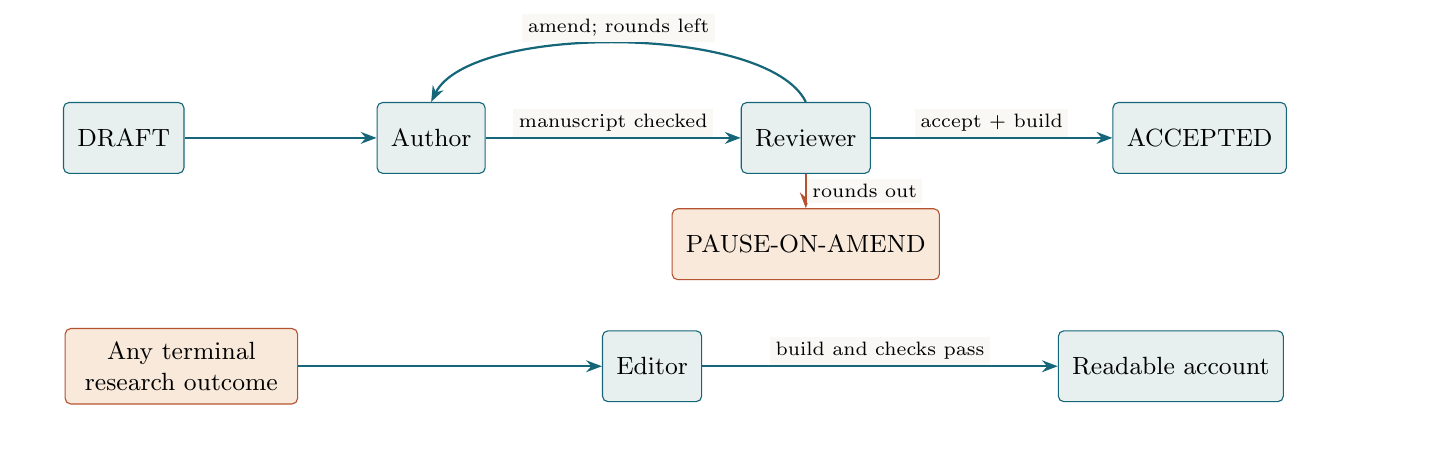
\begin{tikzpicture}[x=1.22cm,y=1cm]
  \path[use as bounding box] (0,-.4) rectangle (14.5,4.6);
  \node[state] (draft) at (1,3.2) {DRAFT};
  \node[state] (author) at (4.2,3.2) {Author};
  \node[state] (review) at (8.1,3.2) {Reviewer};
  \node[state] (accepted) at (12.2,3.2) {ACCEPTED};
  \draw[flow] (draft)--(author);
  \draw[flow] (author)--node[lab,above]{manuscript checked}(review);
  \draw[flow] (review)--node[lab,above]{accept + build}(accepted);
  \draw[flow] (review.north) .. controls (7.7,4.65) and (4.6,4.65) ..
    node[lab,above]{amend; rounds left}(author.north);
  \node[paused] (amend) at (8.1,1.85) {PAUSE-ON-AMEND};
  \draw[flow,draw=Rust] (review)--node[lab,right]{rounds out}(amend);
  \node[paused,text width=2.6cm] (terminal) at (1.6,.3) {Any terminal\\research outcome};
  \node[state] (editor) at (6.5,.3) {Editor};
  \node[state] (account) at (11.9,.3) {Readable account};
  \draw[flow] (terminal)--(editor);
  \draw[flow] (editor)--node[lab,above]{build and checks pass}(account);
\end{tikzpicture}
\takeaway{Acceptance refers to the reviewed manuscript version. Neither output branch silently reopens research.}
\note{Backup. Build and reference failures can trigger bounded repairs or an operational blockage.
Those branches are omitted from this diagram for readability. The full note specifies them and
provides conformance tests. Increasing an allowance does not itself reopen a terminal investigation;
an owner continuation should preserve the previous outcome and record its new scope.}
\end{frame}

\begin{frame}[t]{Backup: what Q4P6 actually assumes}
\paperpair{\Qfour}{\Psix}
\begin{itemize}
  \item Truthful reporting under Q4's own incentive and belief assumptions.
  \item Observers are better than chance, with stable symmetric errors.
  \item Their errors are conditionally independent on the same latent comparison.
  \item Overlapping observations contain a calibration triangle and connect onward.
  \item The agent-comparison graph is connected; the ranking model is specified.
\end{itemize}
\vspace{3mm}\takeaway{A population-identification result, not a finite-sample guarantee or a theorem that these conditions arise automatically.}
\note{Backup. Pairwise observer moments factor as products of reliabilities. A triangle fixes
positive reliabilities, connected overlaps propagate them, and corrected means identify pairwise
comparison probabilities. The Bradley--Terry model then yields contribution scores up to an additive
constant. These are established calibration ingredients used in a conditional interface, not a new
universal identification method. Private peer beliefs, calibration bootstrapping and causal meanings
of contribution remain separate issues.}
\end{frame}

\begin{frame}[t]{Backup: what the dollar scenario does and does not say}
\kicker{Original 330-call cohort; later runs excluded}
\begin{center}\small
\begin{tabular}{lrrr}
\toprule
Stage & Calls & Summed call time & Scenario USD\\
\midrule
Scan & 106 & 18.3 min & \ScanCost\\
Research + consolidation + verification & 168 & 6.07 h & \ResearchCost\\
Manuscript preparation + review & 38 & 1.23 h & \ManuscriptCost\\
Readable accounts & 17 & 28.7 min & \AccountCost\\
Probe & 1 & 4.4 s & 0.13\\
\bottomrule
\end{tabular}\end{center}
\vspace{2mm}
{\small GPT-6 Standard, per million tokens: input \$10; cache read \$1; cache write \$12.50; output \$50.}
\vspace{2mm}
\takeaway{Only input and output counters were retained in these receipts. Missing cache and per-request context data prevent exact normalisation.}
\vspace{2mm}\smallprint{Scenario applies \$10/M and \$50/M to recorded counters only. Above 272K input tokens,
the full request has higher rates. Medium effort is not a multiplier that reconstructs a counterfactual run.}
\note{Backup. The displayed stage values are an arithmetic scenario, not actual model charges.
Claude input counters exclude unrecorded cache activity; Codex input may include cached tokens.
Consequently the missing terms do not have a known net direction. A correct future cost logger
needs disjoint uncached input, cache reads, cache writes, billed output including reasoning,
request-level context length, and separately billed tools. Source: OpenAI model pricing checked
16 September 2026, and the original root receipts frozen into the slide assets.}
\end{frame}

\begin{frame}[t]{Backup: why did we pause?}
\kicker{Proposed review distinction, separate from the stopping mechanism}
\begin{columns}[T,onlytextwidth]
\begin{column}{.48\textwidth}
  \begin{beamercolorbox}[sep=9pt,wd=\linewidth]{paperbox}
    {\Large\color{Teal}PAUSE-PLUS}\par\vspace{3mm}
    An actionable continuation exists.\par\vspace{3mm}
    Name the missing material or experiment, the next step, and what its outcomes would establish.
  \end{beamercolorbox}
\end{column}
\begin{column}{.48\textwidth}
  \begin{beamercolorbox}[sep=9pt,wd=\linewidth]{conclusion}
    {\Large\color{Rust}PAUSE-MINUS}\par\vspace{3mm}
    Evidence undermines this direction.\par\vspace{3mm}
    Explain what was ruled out and why, without claiming that every possible connection is exhausted.
  \end{beamercolorbox}
\end{column}
\end{columns}
\vspace{5mm}\takeaway{An exhausted iteration budget is a stopping reason, not a scientific assessment. Allow ``undetermined'' too.}
\note{Backup. This is a proposed addition to the final review, not a claim that the implementation
already has these states. The two dimensions should remain separate: where the runner stopped,
and what the researchers learned about the prospects of continuing. PAUSE-PLUS must name an
actionable next step; vague optimism is insufficient. Budget exhaustion may leave the assessment undetermined.}
\end{frame}
\end{document}
